\documentclass{standalone}
\usepackage{tikz}
\usetikzlibrary{patterns, positioning}

\begin{document}
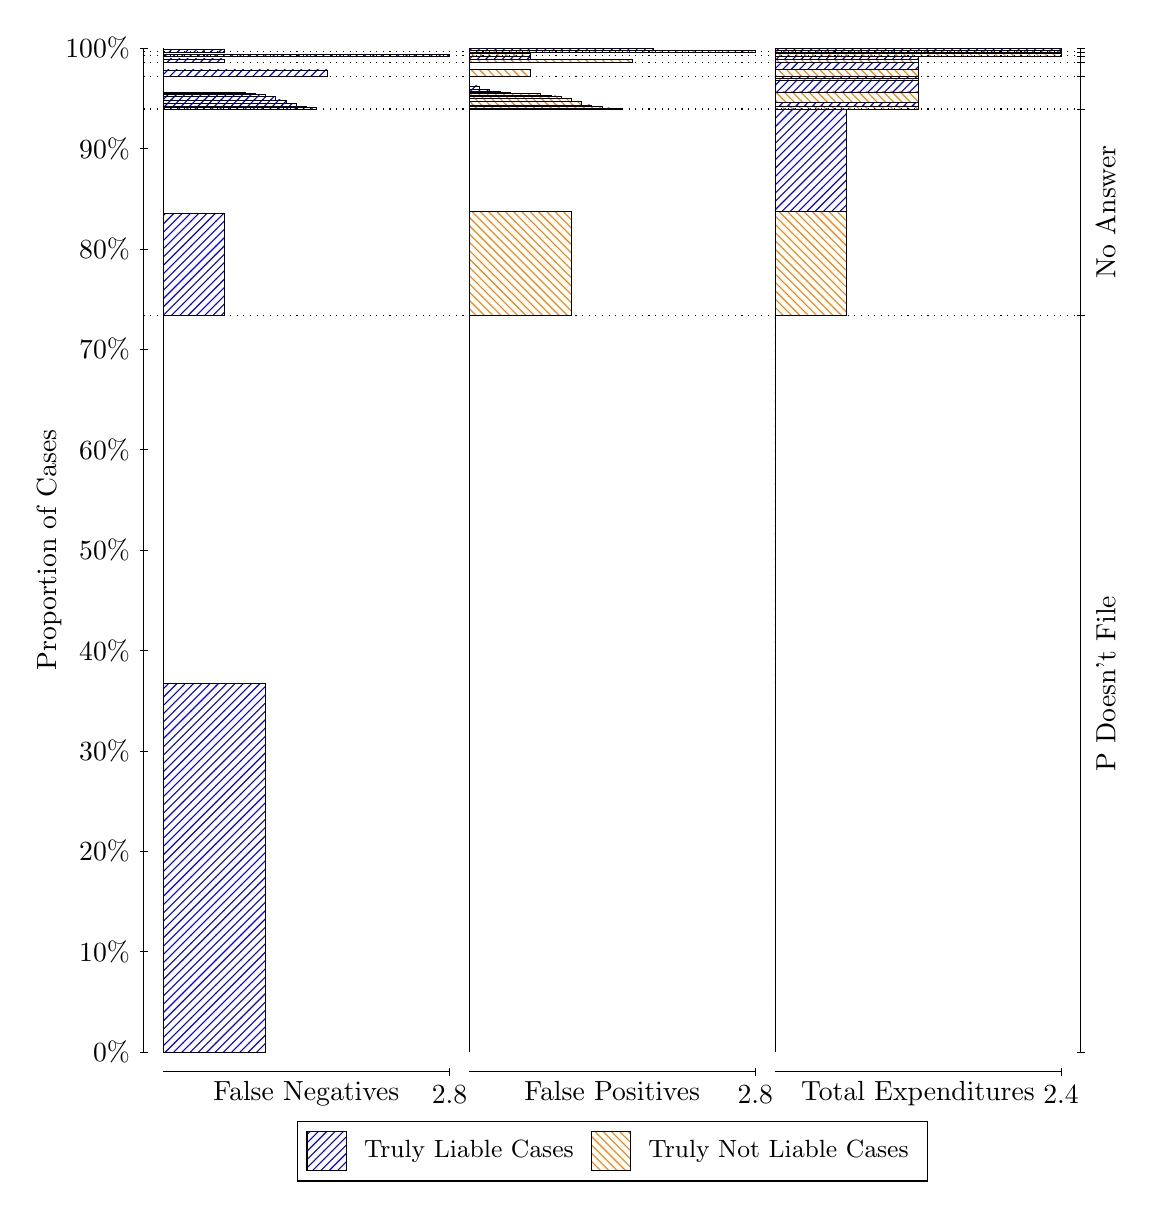
\begin{tikzpicture}
\draw[black, very thin] (1.5,1.75) -- (1.5,14.5);
\node[rotate=90, anchor=center] at (0.3, 8.125) {Proportion of Cases};
\draw[black, very thin] (1.45,1.75) -- (1.55,1.75);
\node[anchor=east] at (1.45, 1.75) {0\%};
\draw[black, very thin] (1.45,3.025) -- (1.55,3.025);
\node[anchor=east] at (1.45, 3.025) {10\%};
\draw[black, very thin] (1.45,4.3) -- (1.55,4.3);
\node[anchor=east] at (1.45, 4.3) {20\%};
\draw[black, very thin] (1.45,5.575) -- (1.55,5.575);
\node[anchor=east] at (1.45, 5.575) {30\%};
\draw[black, very thin] (1.45,6.85) -- (1.55,6.85);
\node[anchor=east] at (1.45, 6.85) {40\%};
\draw[black, very thin] (1.45,8.125) -- (1.55,8.125);
\node[anchor=east] at (1.45, 8.125) {50\%};
\draw[black, very thin] (1.45,9.4) -- (1.55,9.4);
\node[anchor=east] at (1.45, 9.4) {60\%};
\draw[black, very thin] (1.45,10.675) -- (1.55,10.675);
\node[anchor=east] at (1.45, 10.675) {70\%};
\draw[black, very thin] (1.45,11.95) -- (1.55,11.95);
\node[anchor=east] at (1.45, 11.95) {80\%};
\draw[black, very thin] (1.45,13.225) -- (1.55,13.225);
\node[anchor=east] at (1.45, 13.225) {90\%};
\draw[black, very thin] (1.45,14.5) -- (1.55,14.5);
\node[anchor=east] at (1.45, 14.5) {100\%};

\draw[black, very thin] (13.4,1.75) -- (13.4,14.5);
\draw[black, very thin] (13.35,1.75) -- (13.45,1.75);
\node[anchor=west] at (13.35, 1.75) {};
\draw[black, very thin] (13.35,11.102) -- (13.45,11.102);
\node[anchor=west] at (13.35, 11.102) {};
\draw[black, very thin] (13.35,13.726) -- (13.45,13.726);
\node[anchor=west] at (13.35, 13.726) {};
\draw[black, very thin] (13.35,14.135) -- (13.45,14.135);
\node[anchor=west] at (13.35, 14.135) {};
\draw[black, very thin] (13.35,14.315) -- (13.45,14.315);
\node[anchor=west] at (13.35, 14.315) {};
\draw[black, very thin] (13.35,14.401) -- (13.45,14.401);
\node[anchor=west] at (13.35, 14.401) {};
\draw[black, very thin] (13.35,14.451) -- (13.45,14.451);
\node[anchor=west] at (13.35, 14.451) {};
\draw[black, very thin] (13.35,14.5) -- (13.45,14.5);
\node[anchor=west] at (13.35, 14.5) {};

\draw[black, very thin, pattern color=blue, pattern=north east lines] (1.75,1.75) rectangle (3.0476,6.4261);
\draw[black, very thin, pattern color=orange, pattern=north west lines] (1.75,6.4261) rectangle (1.75,11.102);
\draw[black, very thin, pattern color=blue, pattern=north east lines] (1.75,11.102) rectangle (2.5286,12.404);
\draw[black, very thin, pattern color=orange, pattern=north west lines] (1.75,12.404) rectangle (1.75,13.726);
\draw[black, very thin, pattern color=blue, pattern=north east lines] (1.75,13.726) rectangle (3.6964,13.745);
\draw[black, very thin, pattern color=blue, pattern=north east lines] (1.75,13.745) rectangle (3.5667,13.757);
\draw[black, very thin, pattern color=blue, pattern=north east lines] (1.75,13.757) rectangle (3.4369,13.799);
\draw[black, very thin, pattern color=blue, pattern=north east lines] (1.75,13.799) rectangle (3.3071,13.841);
\draw[black, very thin, pattern color=blue, pattern=north east lines] (1.75,13.841) rectangle (3.1774,13.885);
\draw[black, very thin, pattern color=blue, pattern=north east lines] (1.75,13.885) rectangle (3.0476,13.909);
\draw[black, very thin, pattern color=blue, pattern=north east lines] (1.75,13.909) rectangle (2.9179,13.926);
\draw[black, very thin, pattern color=blue, pattern=north east lines] (1.75,13.926) rectangle (2.7881,13.933);
\draw[black, very thin, pattern color=blue, pattern=north east lines] (1.75,13.933) rectangle (2.6583,13.94);
\draw[black, very thin, pattern color=orange, pattern=north west lines] (1.75,13.94) rectangle (1.75,14.135);
\draw[black, very thin, pattern color=blue, pattern=north east lines] (1.75,14.135) rectangle (3.8262,14.223);
\draw[black, very thin, pattern color=orange, pattern=north west lines] (1.75,14.223) rectangle (1.75,14.315);
\draw[black, very thin, pattern color=blue, pattern=north east lines] (1.75,14.315) rectangle (2.5286,14.361);
\draw[black, very thin, pattern color=orange, pattern=north west lines] (1.75,14.361) rectangle (1.75,14.401);
\draw[black, very thin, pattern color=blue, pattern=north east lines] (1.75,14.401) rectangle (5.3833,14.419);
\draw[black, very thin, pattern color=orange, pattern=north west lines] (1.75,14.419) rectangle (1.75,14.451);
\draw[black, very thin, pattern color=blue, pattern=north east lines] (1.75,14.451) rectangle (2.5286,14.482);
\draw[black, very thin, pattern color=orange, pattern=north west lines] (1.75,14.482) rectangle (1.75,14.5);
\draw[black, very thin, pattern color=orange, pattern=north west lines] (5.6333,1.75) rectangle (5.6333,6.4261);
\draw[black, very thin, pattern color=blue, pattern=north east lines] (5.6333,6.4261) rectangle (5.6333,11.102);
\draw[black, very thin, pattern color=orange, pattern=north west lines] (5.6333,11.102) rectangle (6.931,12.425);
\draw[black, very thin, pattern color=blue, pattern=north east lines] (5.6333,12.425) rectangle (5.6333,13.726);
\draw[black, very thin, pattern color=orange, pattern=north west lines] (5.6333,13.726) rectangle (7.5798,13.733);
\draw[black, very thin, pattern color=orange, pattern=north west lines] (5.6333,13.733) rectangle (7.45,13.74);
\draw[black, very thin, pattern color=orange, pattern=north west lines] (5.6333,13.74) rectangle (7.3202,13.756);
\draw[black, very thin, pattern color=orange, pattern=north west lines] (5.6333,13.756) rectangle (7.1905,13.779);
\draw[black, very thin, pattern color=orange, pattern=north west lines] (5.6333,13.779) rectangle (7.0607,13.818);
\draw[black, very thin, pattern color=orange, pattern=north west lines] (5.6333,13.818) rectangle (6.931,13.856);
\draw[black, very thin, pattern color=orange, pattern=north west lines] (5.6333,13.856) rectangle (6.8012,13.891);
\draw[black, very thin, pattern color=orange, pattern=north west lines] (5.6333,13.891) rectangle (6.6714,13.901);
\draw[black, very thin, pattern color=orange, pattern=north west lines] (5.6333,13.901) rectangle (6.5417,13.921);
\draw[black, very thin, pattern color=blue, pattern=north east lines] (5.6333,13.921) rectangle (6.2821,13.928);
\draw[black, very thin, pattern color=blue, pattern=north east lines] (5.6333,13.928) rectangle (6.1524,13.935);
\draw[black, very thin, pattern color=blue, pattern=north east lines] (5.6333,13.935) rectangle (6.0226,13.952);
\draw[black, very thin, pattern color=blue, pattern=north east lines] (5.6333,13.952) rectangle (5.8929,13.976);
\draw[black, very thin, pattern color=blue, pattern=north east lines] (5.6333,13.976) rectangle (5.7631,14.02);
\draw[black, very thin, pattern color=blue, pattern=north east lines] (5.6333,14.02) rectangle (5.6333,14.135);
\draw[black, very thin, pattern color=orange, pattern=north west lines] (5.6333,14.135) rectangle (6.4119,14.227);
\draw[black, very thin, pattern color=blue, pattern=north east lines] (5.6333,14.227) rectangle (5.6333,14.315);
\draw[black, very thin, pattern color=orange, pattern=north west lines] (5.6333,14.315) rectangle (7.7095,14.355);
\draw[black, very thin, pattern color=blue, pattern=north east lines] (5.6333,14.355) rectangle (6.4119,14.401);
\draw[black, very thin, pattern color=orange, pattern=north west lines] (5.6333,14.401) rectangle (6.4119,14.433);
\draw[black, very thin, pattern color=blue, pattern=north east lines] (5.6333,14.433) rectangle (5.6333,14.451);
\draw[black, very thin, pattern color=orange, pattern=north west lines] (5.6333,14.451) rectangle (9.2667,14.468);
\draw[black, very thin, pattern color=blue, pattern=north east lines] (5.6333,14.468) rectangle (7.969,14.5);
\draw[black, very thin, pattern color=orange, pattern=north west lines] (9.5167,1.75) rectangle (9.5167,6.4261);
\draw[black, very thin, pattern color=blue, pattern=north east lines] (9.5167,6.4261) rectangle (9.5167,11.102);
\draw[black, very thin, pattern color=orange, pattern=north west lines] (9.5167,11.102) rectangle (10.425,12.425);
\draw[black, very thin, pattern color=blue, pattern=north east lines] (9.5167,12.425) rectangle (10.425,13.726);
\draw[black, very thin, pattern color=orange, pattern=north west lines] (9.5167,13.726) rectangle (11.333,13.766);
\draw[black, very thin, pattern color=blue, pattern=north east lines] (9.5167,13.766) rectangle (11.333,13.81);
\draw[black, very thin, pattern color=orange, pattern=north west lines] (9.5167,13.81) rectangle (11.333,13.943);
\draw[black, very thin, pattern color=blue, pattern=north east lines] (9.5167,13.943) rectangle (11.333,14.089);
\draw[black, very thin, pattern color=orange, pattern=north west lines] (9.5167,14.089) rectangle (11.333,14.111);
\draw[black, very thin, pattern color=blue, pattern=north east lines] (9.5167,14.111) rectangle (11.333,14.135);
\draw[black, very thin, pattern color=orange, pattern=north west lines] (9.5167,14.135) rectangle (11.333,14.227);
\draw[black, very thin, pattern color=blue, pattern=north east lines] (9.5167,14.227) rectangle (11.333,14.315);
\draw[black, very thin, pattern color=orange, pattern=north west lines] (9.5167,14.315) rectangle (11.333,14.355);
\draw[black, very thin, pattern color=blue, pattern=north east lines] (9.5167,14.355) rectangle (11.333,14.401);
\draw[black, very thin, pattern color=orange, pattern=north west lines] (9.5167,14.401) rectangle (13.15,14.433);
\draw[black, very thin, pattern color=blue, pattern=north east lines] (9.5167,14.433) rectangle (13.15,14.451);
\draw[black, very thin, pattern color=orange, pattern=north west lines] (9.5167,14.451) rectangle (13.15,14.468);
\draw[black, very thin, pattern color=blue, pattern=north east lines] (9.5167,14.468) rectangle (13.15,14.5);
\draw[black, dotted] (1.5,11.102) -- (13.4,11.102);
\draw[black, dotted] (1.5,13.726) -- (13.4,13.726);
\draw[black, dotted] (1.5,14.135) -- (13.4,14.135);
\draw[black, dotted] (1.5,14.315) -- (13.4,14.315);
\draw[black, dotted] (1.5,14.401) -- (13.4,14.401);
\draw[black, dotted] (1.5,14.451) -- (13.4,14.451);
\draw[black, very thin] (1.75,1.5) -- (5.3833,1.5);
\node[anchor=north] at (3.5667, 1.5) {False Negatives};
\draw[black, very thin] (5.3833,1.45) -- (5.3833,1.55);
\node[anchor=north] at (5.3833, 1.45) {2.8};

\draw[black, very thin] (5.6333,1.5) -- (9.2667,1.5);
\node[anchor=north] at (7.45, 1.5) {False Positives};
\draw[black, very thin] (9.2667,1.45) -- (9.2667,1.55);
\node[anchor=north] at (9.2667, 1.45) {2.8};

\draw[black, very thin] (9.5167,1.5) -- (13.15,1.5);
\node[anchor=north] at (11.333, 1.5) {Total Expenditures};
\draw[black, very thin] (13.15,1.45) -- (13.15,1.55);
\node[anchor=north] at (13.15, 1.45) {2.4};

\node[black, centered, rotate=90] at (13.72, 6.4261) {P Doesn't File};
\node[black, centered, rotate=90] at (13.72, 12.414) {No Answer};






\draw (7.449999999999999,1.5) node[draw=none] (baseCoordinate) {};
\begin{scope}[align=center]
        \matrix[scale=0.5, draw=black, below=0.5cm of baseCoordinate, nodes={draw}, column sep=0.1cm]{
            \node[rectangle, draw, minimum width=0.5cm, minimum height=0.5cm, pattern=north east lines, pattern color=blue] {}; &
            \node[draw=none, font=\small] (B) {Truly Liable Cases}; &
            \node[rectangle, draw, minimum width=0.5cm, minimum height=0.5cm, pattern=north west lines, pattern color=orange] {}; &
            \node[draw=none, font=\small] (B) {Truly Not Liable Cases}; \\
            };
\end{scope}

\end{tikzpicture}
\end{document}